\chapter{Compression Algorithms Benchmarking}
\label{chapter:compression_algorithms_benchmark}


\begin{introduction}
    This chapter presents the benchmarking process and results of various compression algorithms. The benchmarking focuses on measuring the time increase in compression and decompression, as well as the compression ratio. By gathering these metrics, we aim to explore any correlation between the time increase and the number of operations performed by each algorithm.

    The results of the benchmarking process provide insights into the performance of the compression algorithms and their suitability for different scenarios. These findings contribute to the understanding of the compression algorithms, enabling us to determine the values to be used for parameters in the energy model. The parameters we aim to determine are the compression ratio ($c_{ration}$), the added compression time increase ($c_{t\_cost}$) and the added decompression time increase ($d_{t\_cost}$).
\end{introduction}

\section{Description of the work}
        The aspects of the compression algorithms that are needed to benchmark are the time increase in compression and decompression and the compression ratio. To gather this data we used the \texttt{perf} profiler to measure the time elapsed, the number of cycles and the number of instructions executed during the compression and decompression of the files. These metrics were gathered to see if there existed any correlation between the time increase and the number of operations each algorithm performed. 
        
        The compression ratio was calculated by dividing the size of the original file by the size of the compressed file. 

\section{Methodology}

    The benchmarking process was done by compressing and decompressing a set of files with different sizes and types. There were three types of files considered:
    \begin{itemize}
        \item Text files, which where gathered from the Project Gutenberg website \url{https://www.gutenberg.org/}.
        Several books were concatenated to create files of approximately 1, 10, 100 and 1000 Megabytes.
        \item Random text files, these are randomly generated text files using the \texttt{/dev/urandom} file, which is a file that generates random data. The sizes of these files are the same as the text files.
        \item Genome sequence files, which were gathered from the NCBI website \url{https://www.ncbi.nlm.nih.gov/}. These sequences are either in the FASTA or FASTQ formats.
    \end{itemize}
    
    The algorithms mentioned in the section \ref{section:compression_algorithms_overview} were used, except for the \texttt{cmix} algorithm due to its large system requirements not making it possible to run on a 16-GB RAM machine. We divided the algorithms into two categories, general purpose and specific. The general purpose algorithms were tested on the text and random text files, while the specific algorithms were tested on the genome sequence files. The \texttt{gzip} algorithm was tested on all files as a way to compare the performance of the specific algorithms.

    % Dizer o porque q se escolheu o gzip para testar todos?

    Each algorithm has a wide set of parameters and tweaks that improve its performance in different scenarios. To make a fair comparison, it was decided to only test the default parameters of each algorithm.

    To account for fluctuations in the system, each algorithm was executed 5 times for each file, and the average of the 5 executions was calculated.

    Due to the large size of files some algorithms would take an unreasonable amount of time to compress and decompress the files, so not every algorithm was tested with every file.
    

\section{Results}

    The results of the benchmarking process are presented in the following sections. We divided the results by the type of algorithm used.

    \subsection{General purpose algorithms}

        As we can see from the following Figures, \ref{fig:text_stats} and \ref{fig:random_text_stats}, independently of the algorithm, the time elapsed, the number of cycles and the number of instructions executed by the algorithms are proportional to the size of the file. This means that the time increase is linear with the size of the file, which is in accordance with the algorithms the compressors use. 

        \begin{figure}[h]
            \centering
            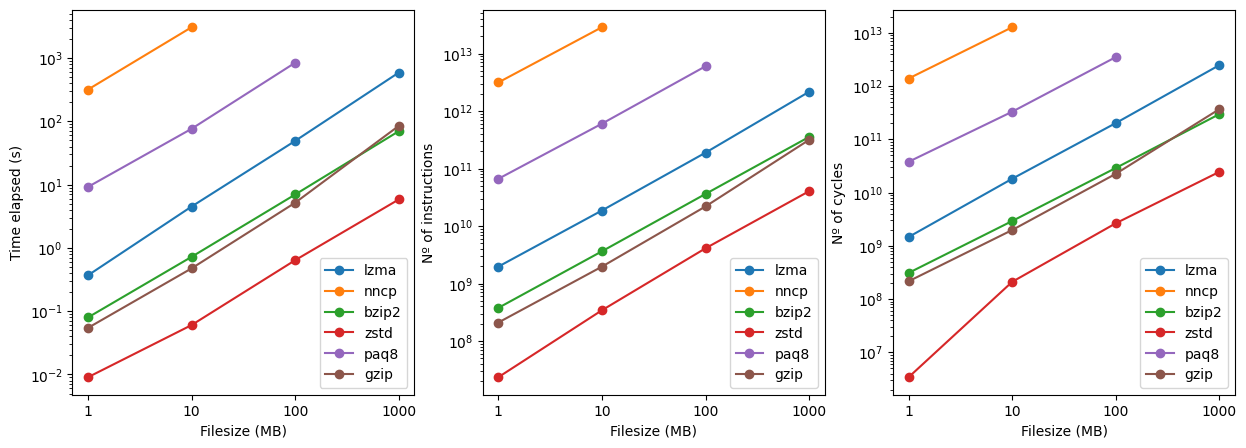
\includegraphics[width=1\textwidth]{figs/text_stats.png}
            \caption[Figure displaying the metrics of the general purpose algorithms when compressing text files.] {Figure displaying the metrics of the general purpose algorithms when compressing text files. The plots display the time elapsed, the number of instructions and the number of cycles executed by the algorithms respectively.}
            \label{fig:text_stats}
        \end{figure}

        \begin{figure}[h]
            \centering
            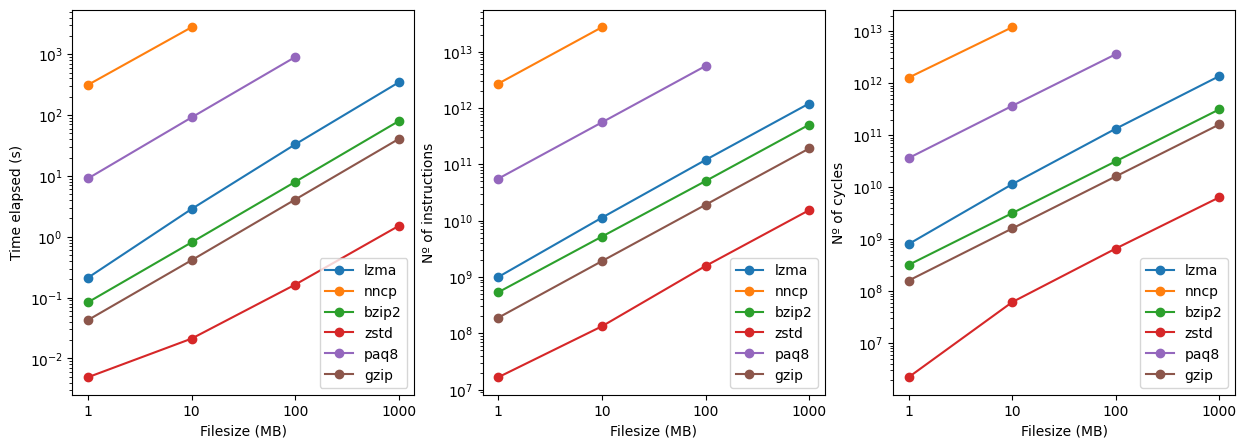
\includegraphics[width=1\textwidth]{figs/random_text_stats.png}
            \caption[Figure displaying the metrics of the general purpose algorithms when compressing random text files.] {Figure displaying the metrics of the general purpose algorithms when compressing random text files. The plots display the time elapsed, the number of instructions and the number of cycles executed by the algorithms respectively.}
            \label{fig:random_text_stats}
        \end{figure}

        Analyzing the metrics we can separate the algorithms into three groups, each separated by at least an order of magnitude in the time metrics.
        The first group comprises solely of \texttt{zstandard}, which proved to be the fastest of the algorithms in all metrics. The second group is composed of \texttt{gzip}, \texttt{bzip2} and \texttt{lzma}, which are the second, third and fourth fastest algorithms, respectively. The third group is composed of the more complex algorithms, such as \texttt{paq8} and \texttt{nncp}, which are the slowest in all metrics. This is expected, as the more complex algorithms need to perform more operations to compress the files.
        
        Changing the type of the file didn't have any significant impact on the time metrics of the algorithms, so time performance isn't related to the data type of the file.

        Observing the compressed size of the files generated by the algorithms, presented in Figures \ref{fig:random_text_comp_size} and \ref{fig:text_comp_size}, and their respectively compression rations, shown in Figures \ref{fig:random_text_comp_ratio} and \ref{fig:text_comp_ratio}, we can see some interesting results. 

        \begin{figure}
            \centering
            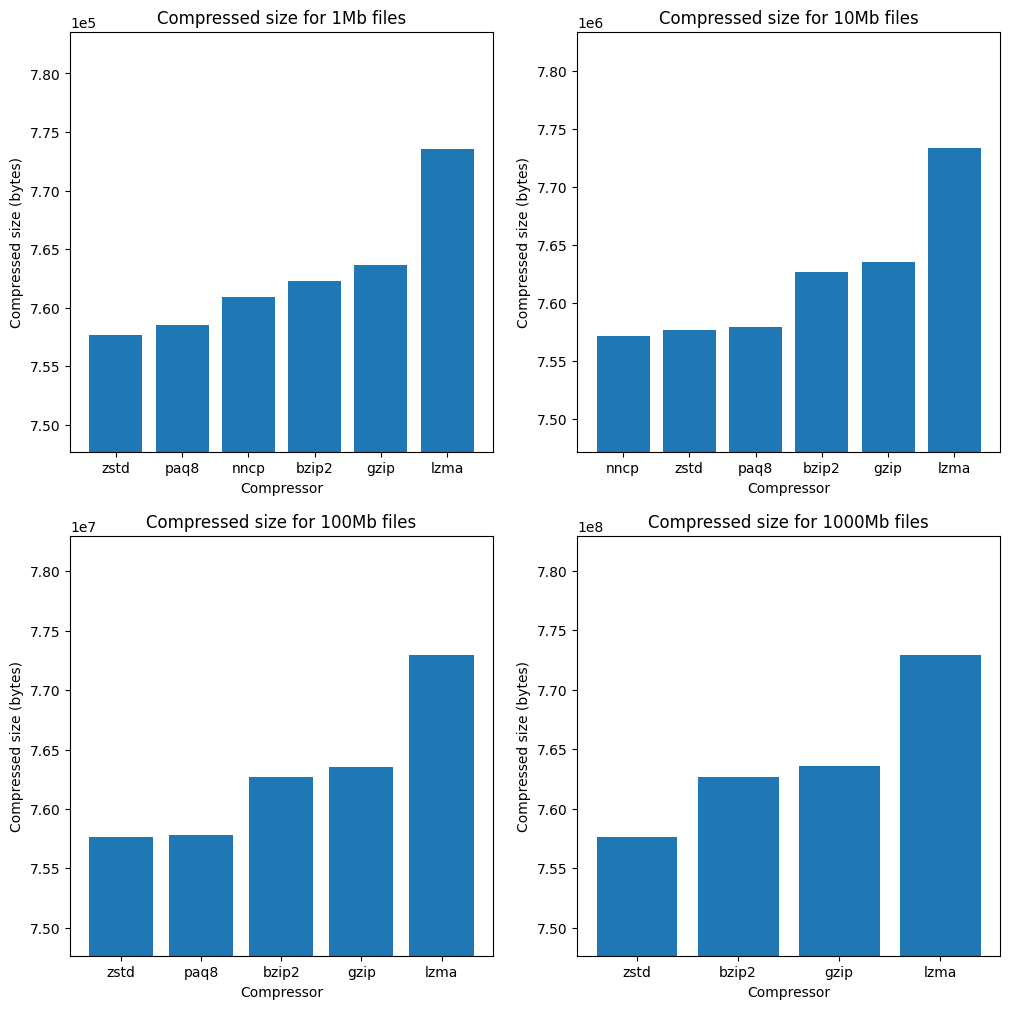
\includegraphics[width=1\textwidth]{figs/random_text_comp_size.png}
            \caption[Figure displaying the size of the compressed files generated by the general purpose algorithms when compressing random text files.] {Figure displaying the size of the compressed files generated by the general purpose algorithms when compressing random text files. Each plot is associated to one of the four text files used in the benchmark.}
            \label{fig:random_text_comp_size}
        \end{figure}

        \begin{figure}
            \centering
            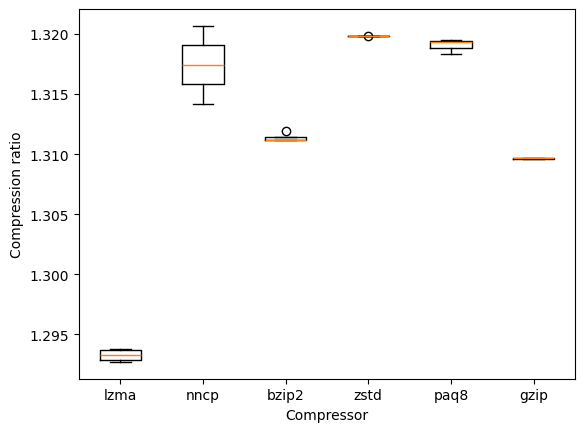
\includegraphics[width=0.5\textwidth]{figs/random_text_comp_ratio.png}
            \caption[Figure displaying the compression ratio of each general purpose compression algorithm for the random text file benchmark.] {Figure displaying the compression ratio of each general purpose compression algorithm for the random text file benchmark.}
            \label{fig:random_text_comp_ratio}
        \end{figure}

        \begin{figure}[h]
            \centering
            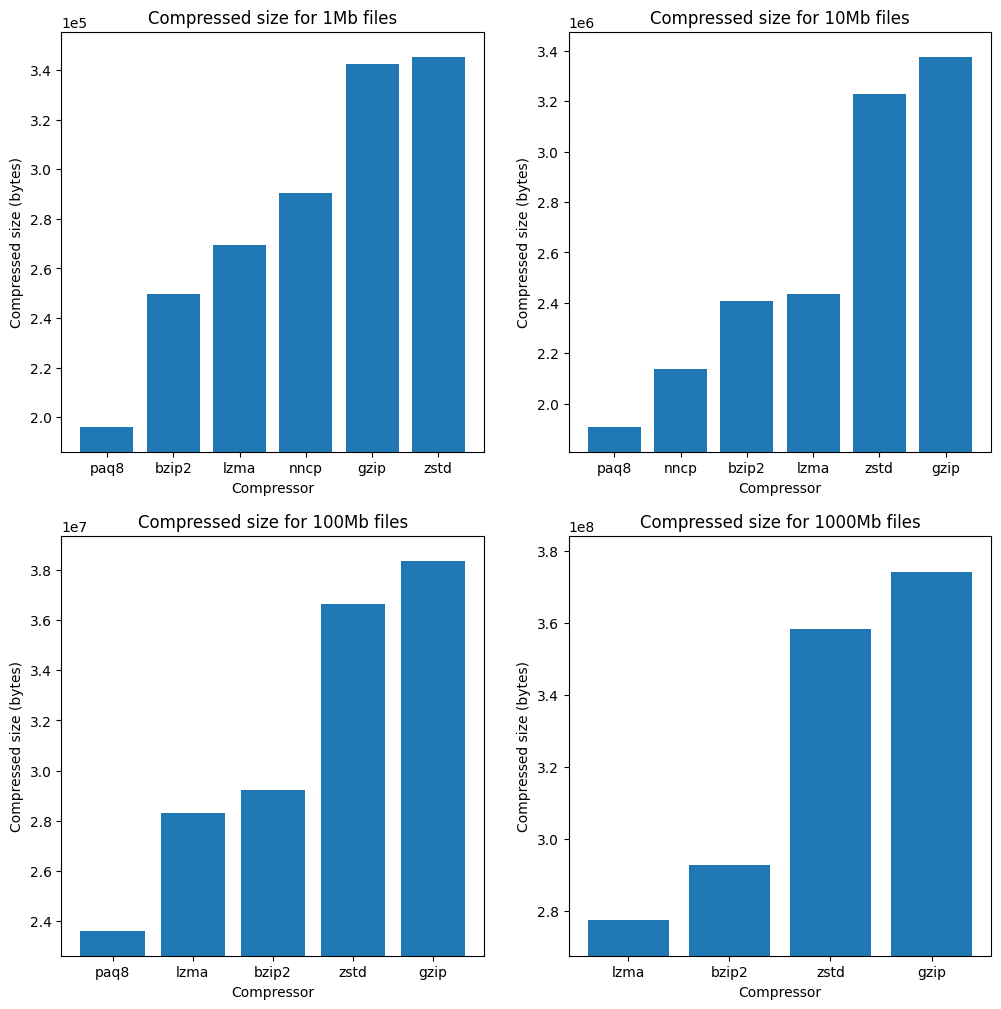
\includegraphics[width=1\textwidth]{figs/text_comp_size.png}
            \caption[Figure displaying the size of the compressed files generated by the general purpose algorithms when compressing text files.] {Figure displaying the size of the compressed files generated by the general purpose algorithms when compressing text files. Each plot is associated to one of the four text files used in the benchmark.}
            \label{fig:text_comp_size}
        \end{figure}

        \begin{figure}[h]
            \centering
            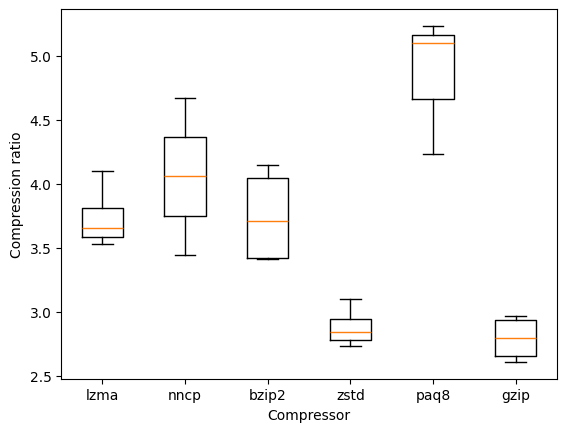
\includegraphics[width=0.5\textwidth]{figs/text_comp_ratio.png}
            \caption[Figure displaying the compression ratio of each general purpose compression algorithm for the text file benchmark.] {Figure displaying the compression ratio of each general purpose compression algorithm for the text file benchmark.}
            \label{fig:text_comp_ratio}
        \end{figure}
        
        First, we see that when dealing with random files, the compression algorithms don't have a good performance, with all algorithms having similar final compressed size, with no one having a ratio higher than 1.4. This means that if the user is expecting to receive a lot of random data, like storing binaries, using compression can be a waste of resources.
        
        Looking at the normal text results, we see that the algorithms that had the fastest metrics in the time benchmarks, \texttt{gzip} and \texttt{zstandard}, also had in general the lowest compression ratios, with both ranking as last and second to last, in almost all file sizes. This means that the algorithms that are faster are also the ones that have the worst compression ratios. This is an interesting trade-off that the user needs to consider when choosing an algorithm.
        Overall, the compression ratio of the algorithms is much better when the contents of the files aren't random, because the algorithms can find patterns in the data to compress.

        The following figures, Figures \ref{fig:text_decomp_stats} and \ref{fig:random_text_decomp_stats} show the results of the decompression metrics. We observe the same rankings as in the compression metrics, with \texttt{zstandard} being the fastest, followed by \texttt{gzip}, \texttt{bzip2} and \texttt{lzma}, and finally \texttt{paq8} being the slowest.
        The growth of the time metrics is also linear with the size of the file for all algorithms, as we can see in the figures. Due to problems with the decompression using \texttt{nncp} we had to exclude it from the benchmarks.


        \begin{figure}[h]
            \centering
            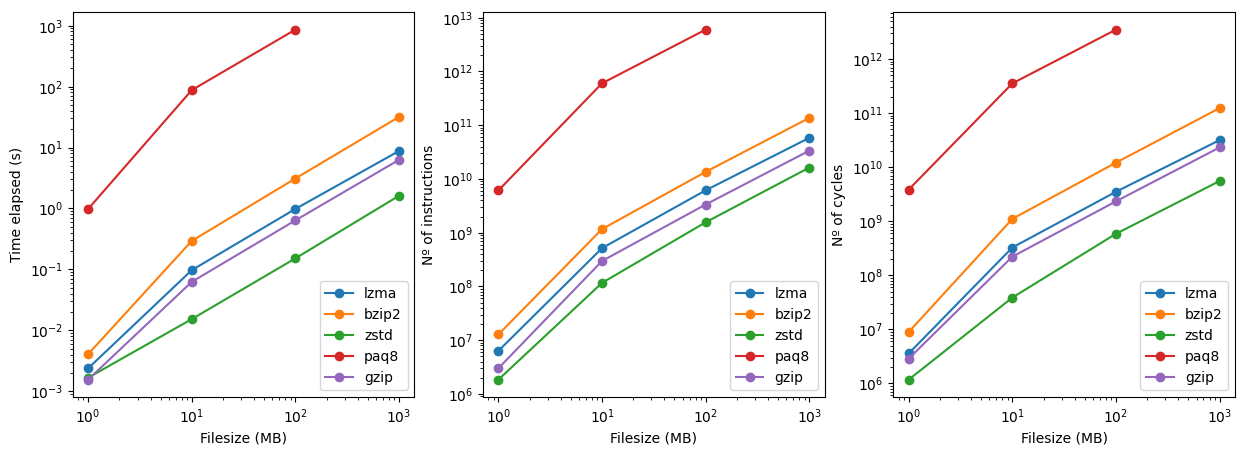
\includegraphics[width=1\textwidth]{figs/text_dstats.png}
            \caption[Figure displaying the metrics of the general purpose algorithms when decompressing text files.] {Figure displaying the metrics of the general purpose algorithms when decompressing text files. The plots display the time elapsed, the number of instructions and the number of cycles executed by the algorithms respectively.}
            \label{fig:text_dstats}
        \end{figure}

        \begin{figure}[h]
            \centering
            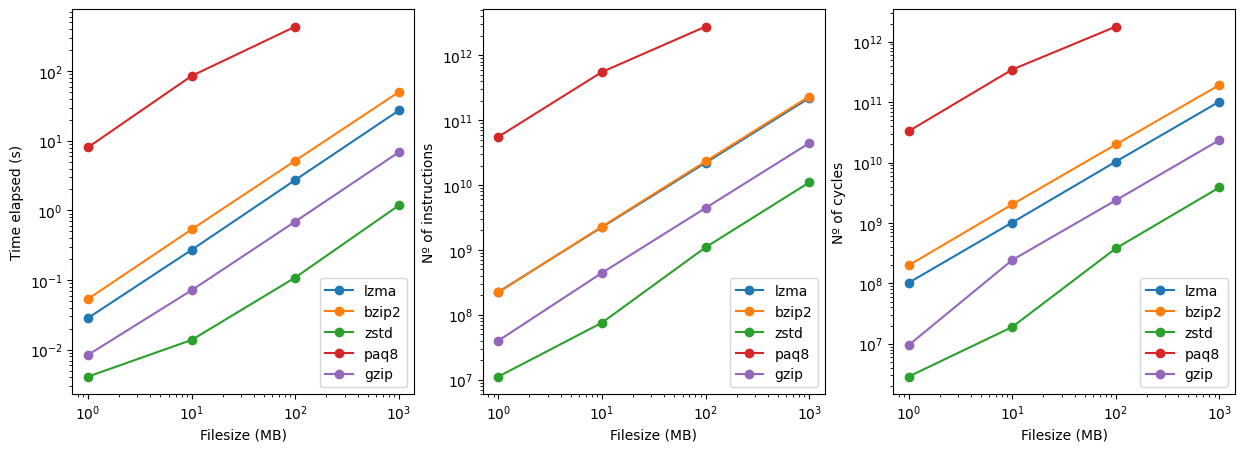
\includegraphics[width=1\textwidth]{figs/random_text_dstats.png}
            \caption[Figure displaying the metrics of the general purpose algorithms when decompressing random text files.] {Figure displaying the metrics of the general purpose algorithms when decompressing random text files. The plots display the time elapsed, the number of instructions and the number of cycles executed by the algorithms respectively.}
            \label{fig:random_text_dstats}
        \end{figure}

        With the results of these benchmarks we can determine the values for the general purpose algorithms to be used in the energy model. The values are presented in Table \ref{table:general_purpose_values}. The compression ratio is the median of the compression ratios of the algorithms in the normal text file benchmark, while the compression and decompression time costs were determined using a poly fitting algorithm to the time elapsed data of the normal and random text file benchmark.

    \begin{table}
        \caption{Values for the compression ratio, compression time cost and decompression time cost of the general purpose algorithms.}
        \label{table:general_purpose_values}
        \begin{center}
        \begin{tabular}{|| c | p{3cm} | p{3cm} | p{3cm} ||}
            \hline
            Compressor & Compression ratio $c_{ration}$ & Compression time cost $c_{t\_cost}$ & Decompression time cost $d_{t\_cost}$ \\
            \hline
            \texttt{gzip} & \multicolumn{1}{r|}{2.79} & \multicolumn{1}{r|}{\num{8.59e-2}} & \multicolumn{1}{r||}{\num{6.27e-3}} \\

            \texttt{zstandard} & \multicolumn{1}{r|}{2.89} & \multicolumn{1}{r|}{\textbf{\num{5.82e-3}}} & \multicolumn{1}{r||}{\textbf{\num{1.62e-3}}} \\

            \texttt{bzip2} & \multicolumn{1}{r|}{3.75} & \multicolumn{1}{r|}{\num{6.99e-2}} & \multicolumn{1}{r||}{\num{3.17e-2}} \\

            \texttt{lzma} & \multicolumn{1}{r|}{3.74} & \multicolumn{1}{r|}{\num{5.94e-1}} & \multicolumn{1}{r||}{\num{8.73e-3}} \\

            \texttt{paq8} & \multicolumn{1}{r|}{\textbf{4.86}} & \multicolumn{1}{r|}{\num{8.49e0}} & \multicolumn{1}{r||}{\num{8.61e0}} \\

            \texttt{nncp} & \multicolumn{1}{r|}{4.06} & \multicolumn{1}{r|}{\num{3.06e2}} & \multicolumn{1}{r||}{-} \\
            
            \hline
        \end{tabular}
        \end{center}
    \end{table}


\subsection{Specific algorithms}

    The specific algorithms were divided into two groups for each file type. The first group is the algorithms that are used to compress the genome sequence files in the FASTA format, while the second group is used to compress the genome sequence files in the FASTQ format.

    The results of the benchmarks for the genome sequence files in the FASTA format are presented in Figures \ref{fig:fasta_stats} and \ref{fig:fasta_comp_size}.
    We can see that like the general purpose algorithms, the time metrics of the specific algorithms are proportional to the size of the file, meaning that the time increase is linear with the size of the file. Also to note, that almost all algorithms had a better performance in relation to the time elapsed, than \texttt{gzip}, except for \texttt{MFCompress} which had a slight worse time.
    
    \begin{figure}[h]
        \centering
        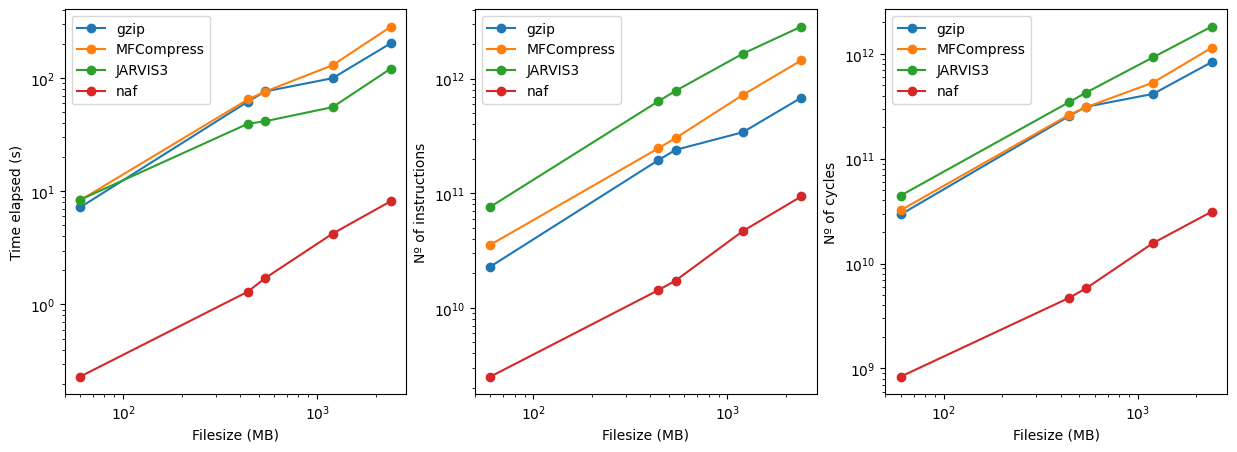
\includegraphics[width=1\textwidth]{figs/fasta_stats.png}
        \caption[Figure displaying the metrics of the specific algorithms when compressing FASTA files.] {Figure displaying the metrics of the specific algorithms when compressing FASTA files. The plots display the time elapsed, the number of instructions and the number of cycles executed by the algorithms respectively.}
        \label{fig:fasta_stats}
    \end{figure}

    \begin{figure}
        \centering
        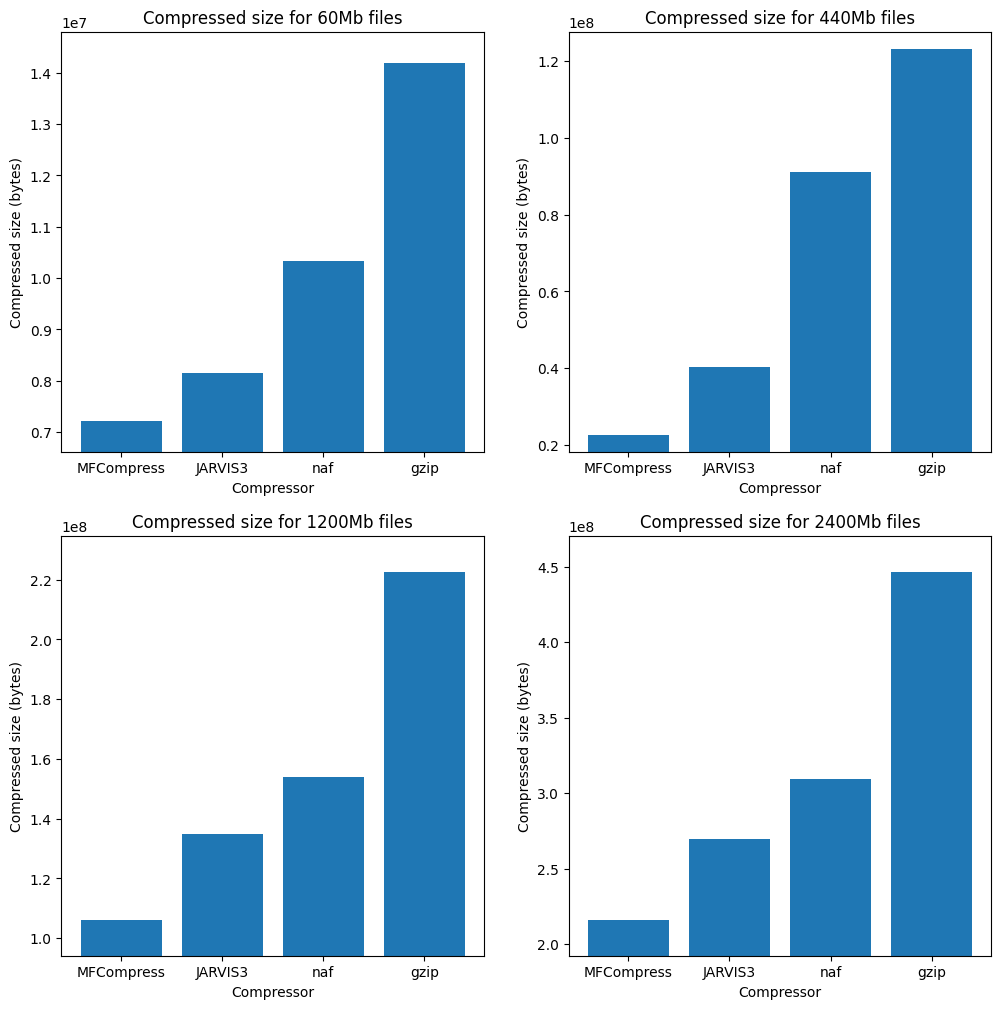
\includegraphics[width=1\textwidth]{figs/fasta_comp_size.png}
        \caption[Figure displaying the size of the compressed files generated by the specific algorithms when compressing FASTA files.] {Figure displaying the size of the compressed files generated by the specific algorithms when compressing FASTA files. Each plot is associated to one of the four text files used in the benchmark.}
        \label{fig:fasta_comp_size}
    \end{figure}

    
    In terms of compression ratio, as expected, all algorithms performed considerably better than \texttt{gzip}. There also exist a correlation with time and compression ratio, with \texttt{MFCompress} having the highest, followed by \texttt{JARVIS3}, and then \texttt{NAF}.

    For the decompression part, Figure \ref{fig:fasta_decomp_stats}, shows that like the compression metrics, the time complexity for decompression is linear with the size of the file. However, the rankings of the algorithms shifts. The new order from fastest to slowest is \texttt{NAF}, \texttt{gzip}, \texttt{JARVIS3} and \texttt{MFCompress}. There exists an irregularity in the time metrics of \texttt{MFCompress}, with the time reducing between 440MB and 540MB, this is due to the multithreading of the algorithm, which is only used when the file is larger than 500MB. 

    \begin{figure}[h]
        \centering
        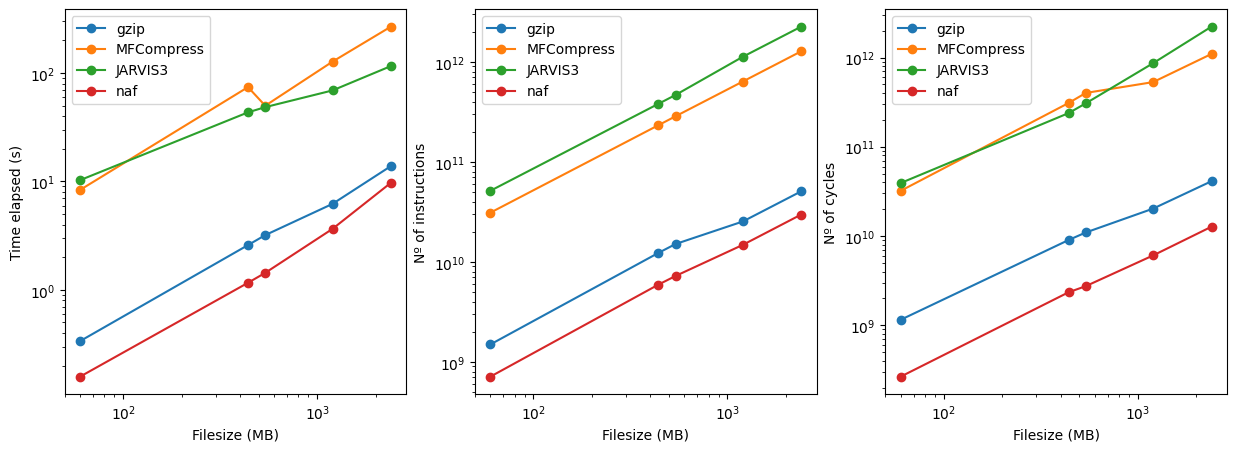
\includegraphics[width=1\textwidth]{figs/fasta_dstats.png}
        \caption[Figure displaying the metrics of the specific algorithms when decompressing FASTA files.] {Figure displaying the metrics of the specific algorithms when decompressing FASTA files. The plots display the time elapsed, the number of instructions and the number of cycles executed by the algorithms respectively.}
        \label{fig:fasta_dstats}
    \end{figure}

    The results of the benchmarks for the genome sequence files in the FASTQ format are presented in Figures \ref{fig:fastq_stats} and \ref{fig:fastq_comp_size}. Like the results for the FASTA files, most compressors presented a linear time growth, except for \texttt{spring}, more data points would be necessary to determine its growth.
    
    \begin{figure}[h]
        \centering
        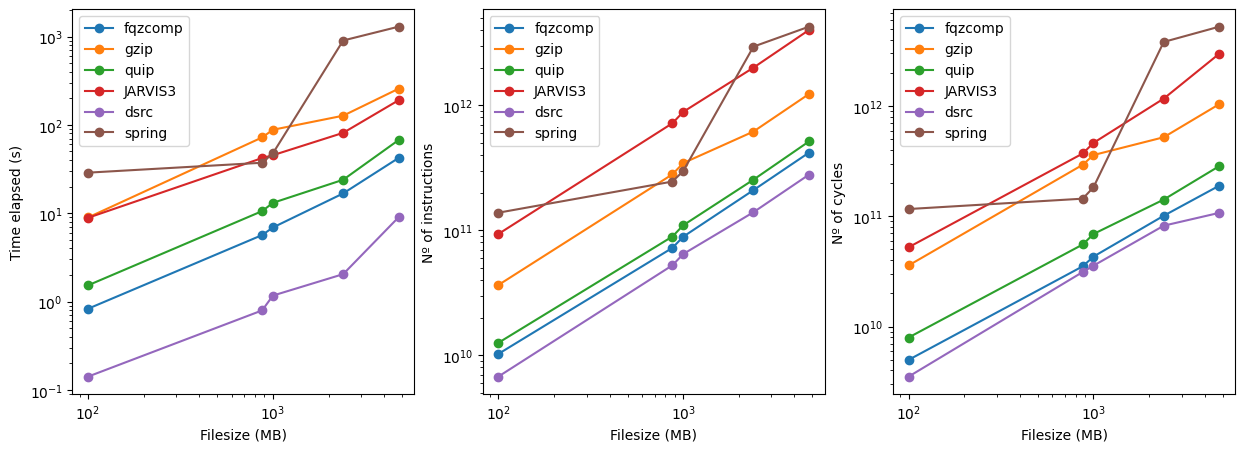
\includegraphics[width=1\textwidth]{figs/fastq_stats.png}
        \caption[Figure displaying the metrics of the specific algorithms when compressing FASTQ files.] {Figure displaying the metrics of the specific algorithms when compressing FASTQ files. The plots display the time elapsed, the number of instructions and the number of cycles executed by the algorithms respectively.}
        \label{fig:fastq_stats}
    \end{figure}

    \begin{figure}
        \centering
        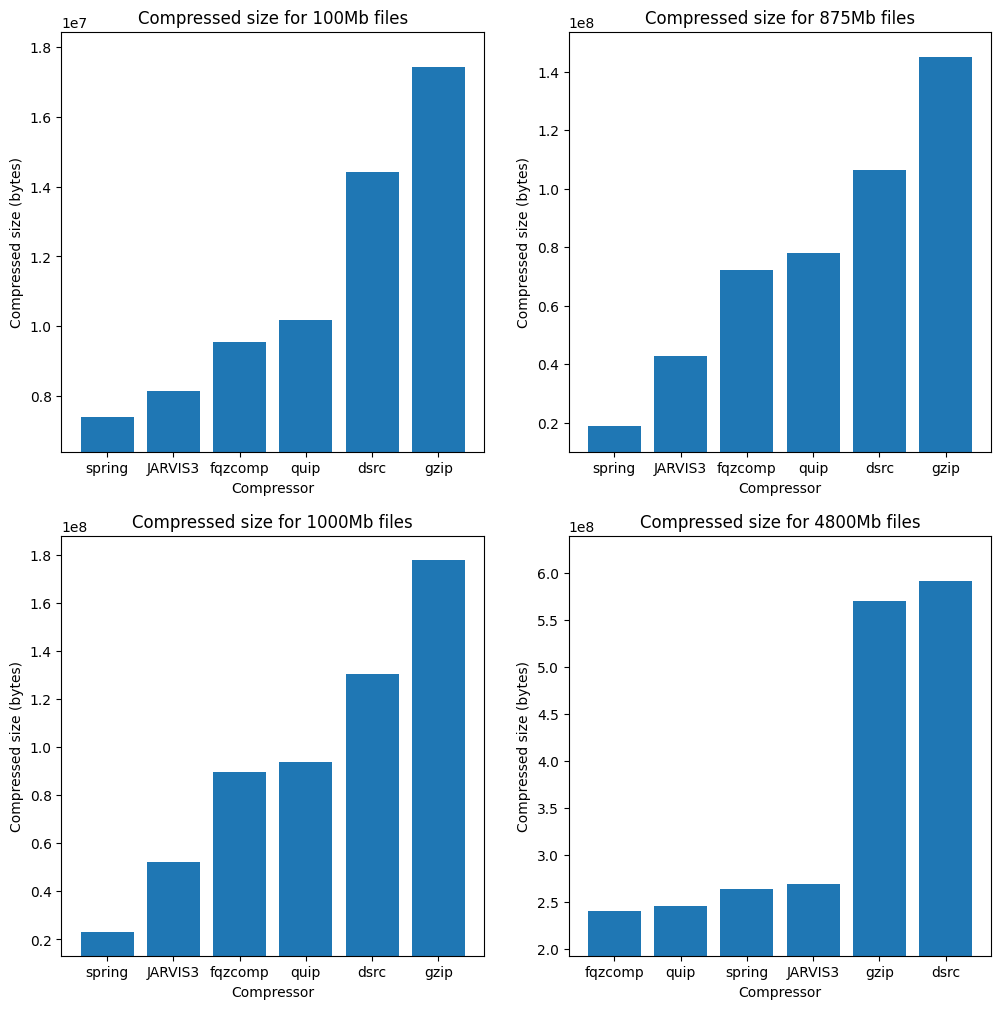
\includegraphics[width=1\textwidth]{figs/fastq_comp_size.png}
        \caption[Figure displaying the size of the compressed files generated by the specific algorithms when compressing FASTQ files.] {Figure displaying the size of the compressed files generated by the specific algorithms when compressing FASTQ files. Each plot is associated to one of the four text files used in the benchmark.}
        \label{fig:fastq_comp_size}
    \end{figure}


    The compression ratio of the specific compressors, was in general a better than \texttt{gzip}, however, \texttt{DSRC} appears to fall-off when larger files are compressed. Nonetheless, the average compression ratio of all algorithms is higher than \texttt{gzip}.

    The decompression metrics are shown in Figure \ref{fig:fastq_dstats}. In terms of time complexity, all the compressors appear to have a linear growth with the size of the file. The rankings of the algorithms also changes, with only \texttt{DSRC} performing better than \texttt{gzip}. The rest algorithms are ranked as follows, \texttt{fqzcomp}, \texttt{quip}, \texttt{spring}, and lastly \texttt{JARVIS3}.

    \begin{figure}[h]
        \centering
        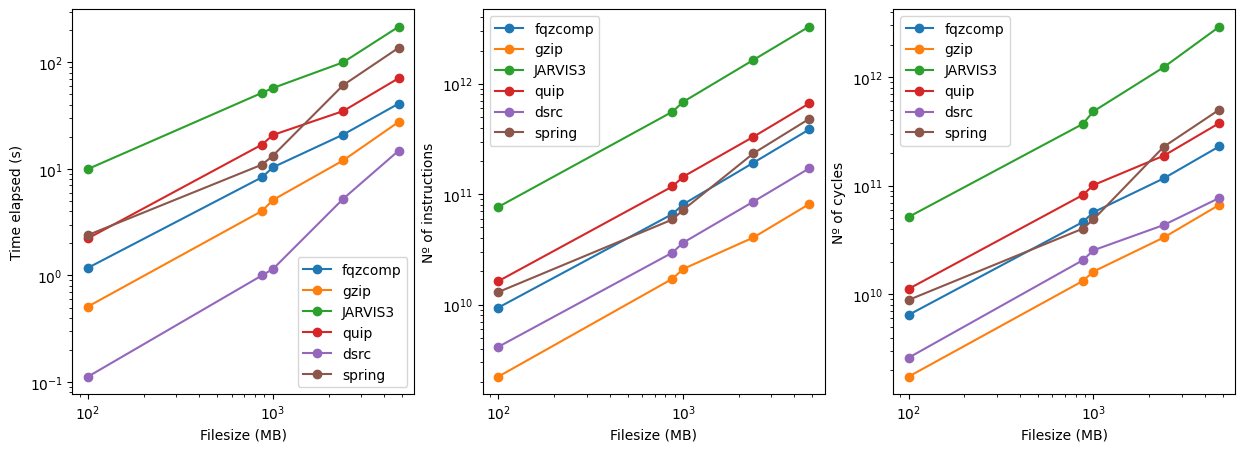
\includegraphics[width=1\textwidth]{figs/fastq_dstats.png}
        \caption[Figure displaying the metrics of the specific algorithms when decompressing FASTQ files.] {Figure displaying the metrics of the specific algorithms when decompressing FASTQ files. The plots display the time elapsed, the number of instructions and the number of cycles executed by the algorithms respectively.}
        \label{fig:fastq_dstats}
    \end{figure}


    In Table \ref{table:specific_values} we show what group each algorithm is part of, as well as the values for the compression ratio, compression time cost and decompression time cost of each compressor.


    \begin{table}
        \caption{Values for the compression ratio, compression time cost and decompression time cost of the specific compressors.}
        \label{table:specific_values}
        \begin{center}
        \begin{tabular}{|| c | c | p{3cm} | p{3cm} | p{3cm} ||}
            \hline
            Compressor & File type & Compression ratio $c_{ration}$ & Compression time cost $c_{t\_cost}$ & Decompression time cost $d_{t\_cost}$ \\
            \hline
            \texttt{gzip} & FASTA & \multicolumn{1}{r|}{4.42} & \multicolumn{1}{r|}{\num{7.72e-2}} & \multicolumn{1}{r||}{\num{5.71e-3}} \\

            \texttt{gzip} & FASTQ & \multicolumn{1}{r|}{6.85} & \multicolumn{1}{r|}{\num{4.93e-2}} & \multicolumn{1}{r||}{5e82e-3} \\

            \texttt{MFCompress} & FASTA & \multicolumn{1}{r|}{13.7} & \multicolumn{1}{r|}{\num{1.15e-1}} & \multicolumn{1}{r||}{\num{1.09e-1}} \\

            \texttt{NAF} & FASTA & \multicolumn{1}{r|}{6.20} & \multicolumn{1}{r|}{\num{3.46e-3}} & \multicolumn{1}{r||}{\num{4.16e-3}} \\

            \texttt{JARVIS3} & FASTA & \multicolumn{1}{r|}{9.44} & \multicolumn{1}{r|}{\num{4.48e-2}} & \multicolumn{1}{r||}{\num{4.416e-2}} \\

            \texttt{JARVIS3} & FASTQ & \multicolumn{1}{r|}{17.5} & \multicolumn{1}{r|}{\num{3.77e-2}} & \multicolumn{1}{r||}{\num{4.25e-2}} \\

            \texttt{DSRC} & FASTQ & \multicolumn{1}{r|}{7.81} & \multicolumn{1}{r|}{\num{1.90e-3}} & \multicolumn{1}{r||}{\num{3.28e-3}} \\

            \texttt{Fqzcomp} & FASTQ & \multicolumn{1}{r|}{14.7} & \multicolumn{1}{r|}{\num{8.92e-3}} & \multicolumn{1}{r||}{\num{8.37e-3}} \\

            \texttt{Quip} & FASTQ & \multicolumn{1}{r|}{14.1} & \multicolumn{1}{r|}{\num{1.39e-2}} & \multicolumn{1}{r||}{\num{1.41e-2}} \\

            \texttt{Spring} & FASTQ& \multicolumn{1}{r|}{27.9} & \multicolumn{1}{r|}{\num{3.07e-1}} & \multicolumn{1}{r||}{\num{3.03e-2}} \\
            
            \hline
        \end{tabular}
        \end{center}
    \end{table}


\section{Conclusions}

    The various compressors evaluated have different trade-offs between time and compression ratio. So there isn't a compressor that is the best for all scenarios, the user needs to evaluate what is more important for their use case.
    
    If the user intends to have a large cold storage, that is, a storage that is rarely accessed, the user should prioritize the compression ratio, as the time increase in compression and decompression won't be a problem. In this case, the user could opt in for the more complex algorithms, like \texttt{paq8} or \texttt{nncp}, that have the best compression ratios. 
    
    On the other hand if the user has a storage that is frequently accessed, the user should prioritize the time increase, as the user will be frequently compressing and decompressing files. In this case, the user should opt in for the faster algorithms, like \texttt{zstandard} or \texttt{gzip}. 

    Another factor to consider is the data type of the files, and use the appropriate compressor for it. Such is the case shown here of the data in the FASTA and FASTQ formats, where the specific compressors had a better performance than the general purpose compressors. 

